\graphicspath{{./assets/}}
\setcounter{mtc}{2}
\chapter{1st Sprint: Preliminary setup of the PaaS infrastructure  }
\fancyhead[R]{\ungaramond\small\textbf{Chapter II. 1st Sprint: Preliminary setup of the PaaS infrastructure }}
\minitoc
\newpage

\section{Sprint backlog :}

\begin{longtable}[H]{|m{1.5cm}|m{3cm}|m{1.5cm}|m{8cm}|}
\hline
{\textbf{EpicID}} & {\textbf{Epic}} & {\textbf{StoryID}} & {\textbf{Story}} \\
\hline
1 &  \raggedright Exploring assets.	& 1.1  & SCM structuring: service components need to be split into different repos. \\
\cline{3-4}
& & 1.2 &  	Keeping track of developed applications and their requirements \\
\hline
2  & Maintenance. &	2.1	 &  Rebuilding optimized containers for developed applications. \\
\cline{3-4}
& & 2.2 & Backup of existing data on current infrastructure in S3 containers.\\
\hline
\caption{1st sprint Backlog}
\end{longtable}

\section{Overview and maintenance of the existing resources}
\subsection{Maintenance operations}

In this sprint, we have assembled standalone self-hosted services into a single stack of upgraded container versions in order to provide better visibility of workloads. A container management platform was then added to this stack to improve on operability. 
The following figure is the deployment diagram of the resulting docker-compose stack:

 \begin{figure}[H] 
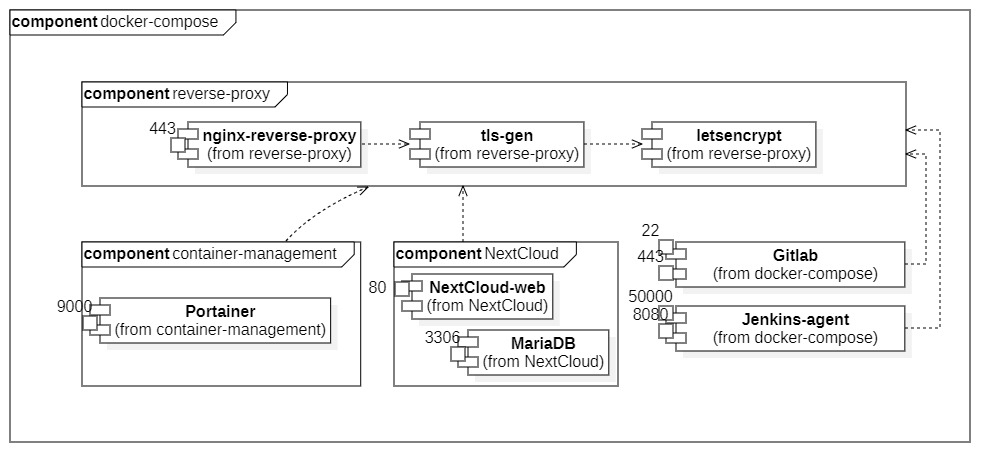
\includegraphics[width=1.0\textwidth,angle=00]{assets/f9.jpg}
\caption{PaaS infrastructure}
\label{fig:f9}
\end{figure}

The stack includes the following services: 
\begin{enumerate}
\item Nginx reverse proxy: An HTTP server that acts as a reverse proxy for the other services in the stack. It is responsible for routing traffic to the correct service based on the URL and handling HTTPS encryption. It recognizes labels configured in the containers to route traffic and provide tls termination. 
\item TLS generator: A service that generates and renews TLS certificates using Let's Encrypt. It works with Nginx to provide HTTPS encryption for the other services in the stack. 
\item Let's Encrypt: A certificate authority that provides free TLS certificates. 
\item Portainer: A web-based management interface for Docker containers and services. 
\item Nextcloud: A cloud-based file sharing and collaboration platform. 
\item GitLab: A web-based Git repository manager, CI/CD pipeline tool, and issue tracker. 
\item Jenkins: An open source automation server that can be used to automate software build, test, and deployment processes. 
\end{enumerate}

Each service is defined in a separate Docker container and is configured using environment variables, volumes, and ports. The Nginx and TLS generator services depend on each other, and the Nextcloud, GitLab, and Jenkins services depend on the TLS generator for HTTPS encryption. 

This Docker Compose stack provides a scalable and easy-to-manage infrastructure for hosting multiple cloud-based services, all secured using HTTPS encryption and Let's Encrypt TLS certificates. 

\subsection{Application overview and SCM structuring}

Two main applications were in development during this project. We have recommended a better source code management strategy that resulted in separating services into different repos in order to optimize the container image creation process. The resulting deployment diagram Is as follows: 

 \begin{figure}[H]\centering
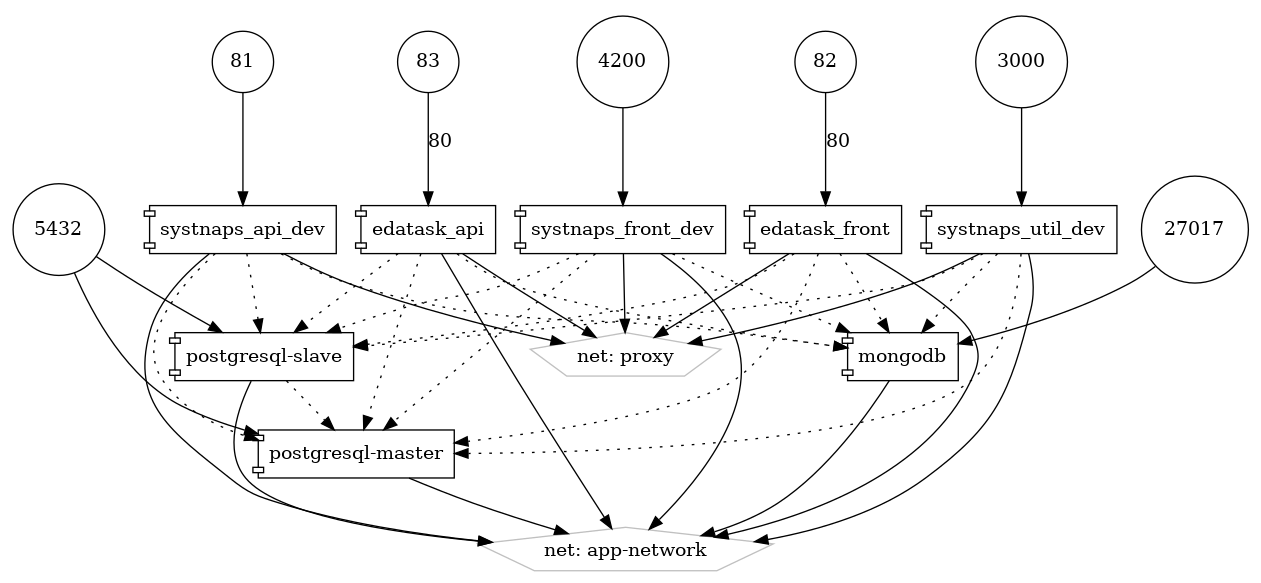
\includegraphics[width=1.0\textwidth,angle=00]{assets/f10.png}
\caption{ Deployment Diagram }
\label{fig:DeploymentDiagram}
\end{figure}

The stack includes the following services: 
\begin{enumerate}
\item Backend API: A Symfony\cite{Symfony} API that serves as the backend for the application. It is responsible for processing requests and returning data to the frontend. 
\item Frontend: An Angular\cite{Angular} web application that serves as the frontend for the application. It is responsible for displaying data and interacting with the backend API. 
\item HA PostgreSQL\cite{PostgreSQL}: A relational database management system that stores data for the application. It is used to store structured data for the backend API. 
\item Replicated MongoDB\cite{MongoDB}: A NoSQL database management system that stores data for the application. It is used to store unstructured data for the frontend. 
\item Nginx\cite{Nginx}: A web server that acts as a reverse proxy for the other services in the stack. It is responsible for routing traffic to the correct service based on the URL and handling HTTPS encryption. 
\end{enumerate}

The backend API, frontend, MongoDB and PostgreSQL are connected using the "app-network" network. All services are also connected to the "proxy" network where Nginx resides, enabling the reverse proxy detect labels and route traffic to the appropriate service based on the URL.
\newpage
\section{Cloud design of the PaaS infrastructure}
\subsection{Package diagram of cloud resources :}

The cluster resources are basically cloud instances with different specifications tailored to their use cases. Three major groups of resources are distinguished in the following diagram: Control plane instances, Compute instances and storage assets which are object store buckets and compute instances to which raw block stores are attached. 

\begin{figure}[H]\centering
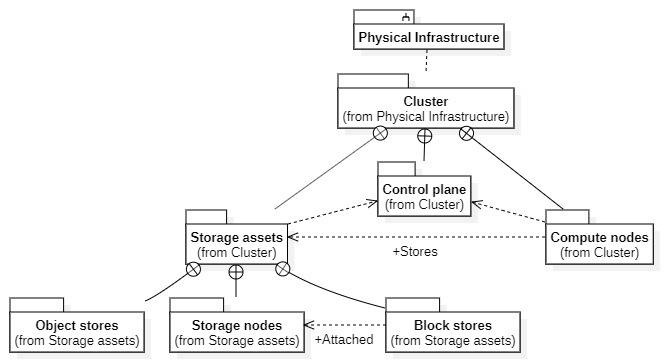
\includegraphics[width=1.0\textwidth,angle=00]{assets/f11.jpg}
\caption{Package diagram of cloud resources }
\label{fig:Package diagram of cloud resources }
\end{figure}

\subsection{Comparative study on container orchestrators: }

Container Orchestration Engines such as “Kubernetes”, “Apache Mesos” and “docker swarm” are platforms for managing containers and automating the deployment, scaling, and operations of containers across a cluster of nodes. This is achieved by pooling the discrete cloud resources into a single PaaS on which workloads can be deployed. 

\begin{longtable}[H]{|m{3.5cm}|m{3.5cm}|m{3.5cm}|m{3.5cm}|}
\hline
Criteria & Kubernetes & Docker swarm & Apache Mesos  \\
\hline
Ease of use & Medium & Easy & Complex  \\
\hline
Cluster scalability & Medium to Large & Small to Medium & Very Large  \\
\hline
Cluster installation & Complex & Easy & Medium  \\
\hline
Container deployment & YAML based  & Docker based & JSON based \\
\hline
Community Support  & Large  & Moderate  & Small \\
\hline
Configuration & Declarative  & Declarative & Imperative \\
\hline
\caption{Sprint planification}
\end{longtable}

Kubernetes is our container orchestration tool of choice in this project. It is known for its highly advanced orchestration capabilities, built-in load balancing, rolling updates, and self-healing. It has a declarative configuration model and a highly extensible architecture. However, it does have a steeper learning curve compared to Docker Swarm.  

Our goal is to tackle the task of establishing a fully sustainable PaaS by utilizing its flexibility via custom resource definitions. 


\subsection{Package diagram for the PaaS logical components:}

\begin{figure}[H]\centering
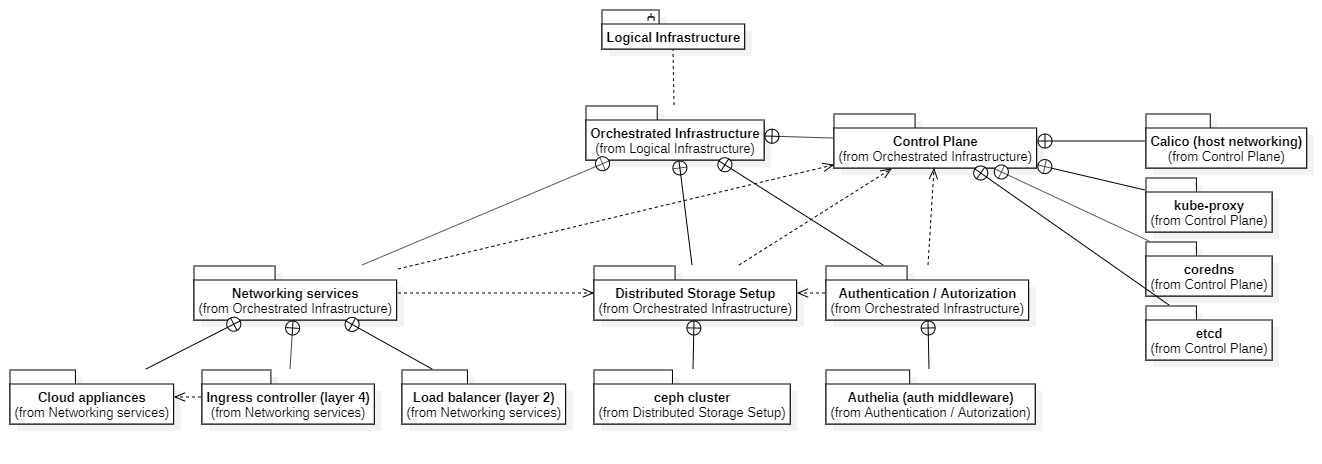
\includegraphics[width=1.0\textwidth,angle=00]{assets/f12.jpg}
\caption{Package diagram for the PaaS logical components}
\label{fig:Package diagram for the PaaS logical components}
\end{figure}

This figure illustrates a package design of the main PaaS services. We mainly distinguish: 
\begin{itemize}[label={--}]
\item  A control plane: which manages assets in the cluster, namely, nodes, pods and other api resources. 
\item An assortment of networking services which allow for ingress control in both the network and application layers. 
\item An authentication and authorization service: which is aimed to control access to the cluster. 
\item A distributed, scalable, and replicated storage backend which is independent of the infrastructure in place to provide data redundancy and disaster recovery. 
\end{itemize}
\newpage
\section{Resource provisiong for the PaaS infrastructure}
\subsection{UML design : class diagram for cloud infrastructure }
The following diagram showcases the interaction between the infrastructure as code tools and the cloud provider as well as the resulting infrastructure, its components, and the relation between them. 
\begin{figure}[H]\centering
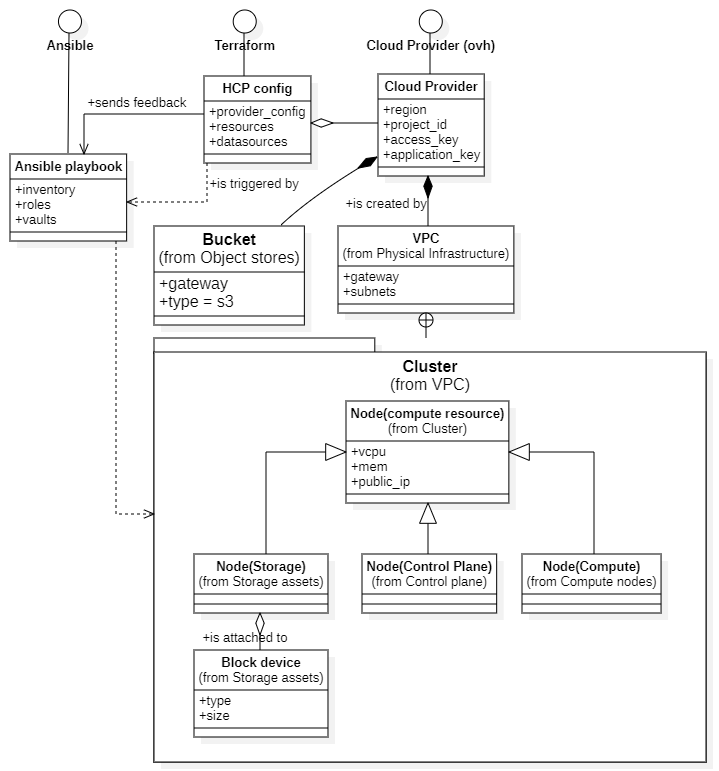
\includegraphics[width=1.0\textwidth,angle=00]{assets/f13.png}
\caption{Class Diagram for cloud infrastructure}
\label{fig:fig13}
\end{figure}

\subsection{“HCP config” diagram for cloud provisioning: }
The following figure illustrates the main resources declared in our terraform “HCP config”: 

\begin{figure}[H]\centering
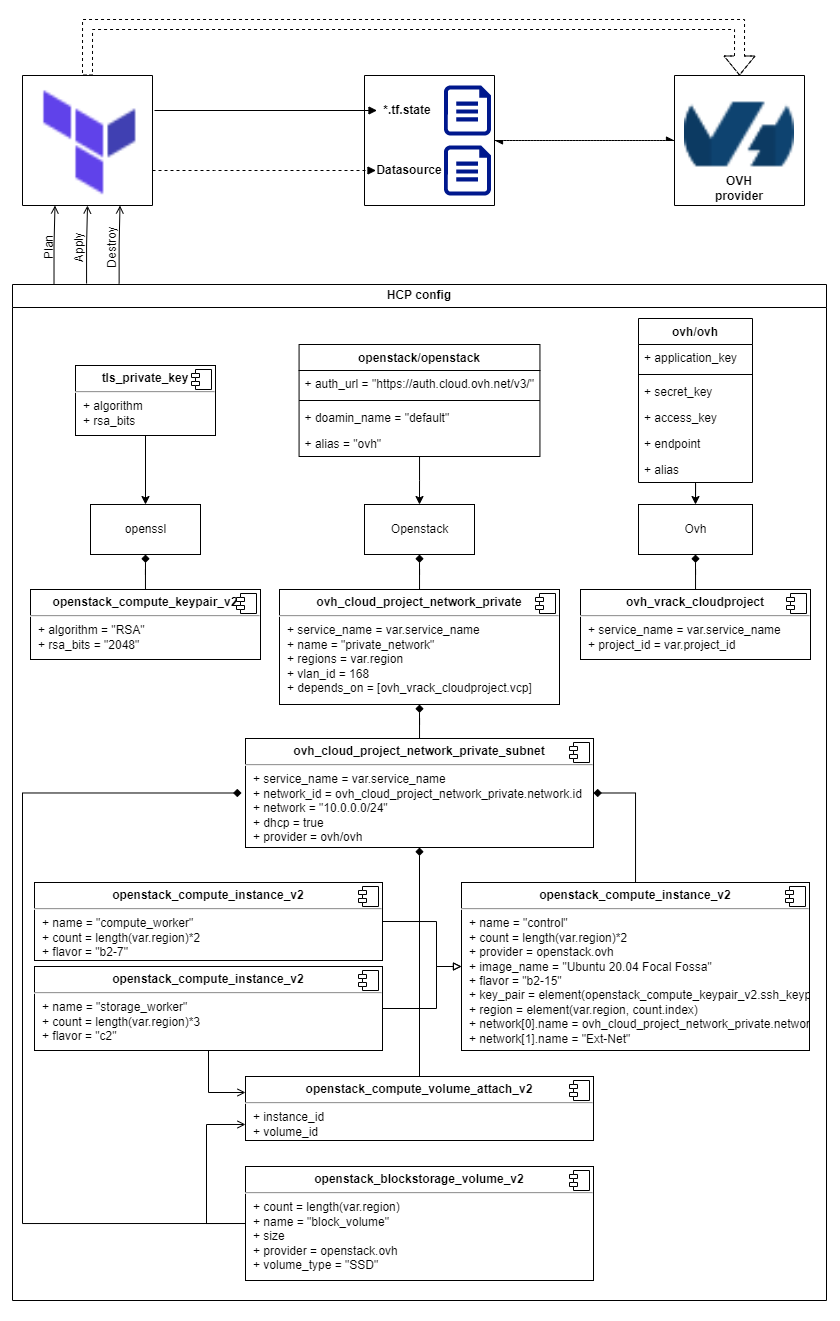
\includegraphics[width=0.8\textwidth]{assets/f14.png}
\caption{Diagram for cloud provisionning}
\label{fig:fig14}
\end{figure}
\newpage
The diagram shows a Terraform configuration for deploying resources on OVH cloud provider. The configuration consists of four main components: provider, network, compute, and storage. 

\begin{itemize}[label={--}]
\item The provider component specifies the OVH cloud provider and the authentication credentials to access the account. 
\item The network component defines the virtual private cloud (VPC) and its associated resources, such as subnets, security groups, and routers. 
\item The compute component defines the public cloud compute instances that will host our PaaS. The VMs are launched in the subnets defined in the network component, and their configurations are specified through variables. 
\item The storage component defines the object storage bucket that will store application and backup data, and the block storage volumes that will be attached to the VMs. 
\end{itemize}

All the resources are managed by Terraform, which allows for easy provisioning, scaling, and management of the infrastructure. 

Overall, this Terraform configuration with OVH cloud provider provides a scalable, secure, and highly available infrastructure for running applications. 

\subsection{Component diagram of provisioned resources}

\begin{figure}[H]\centering
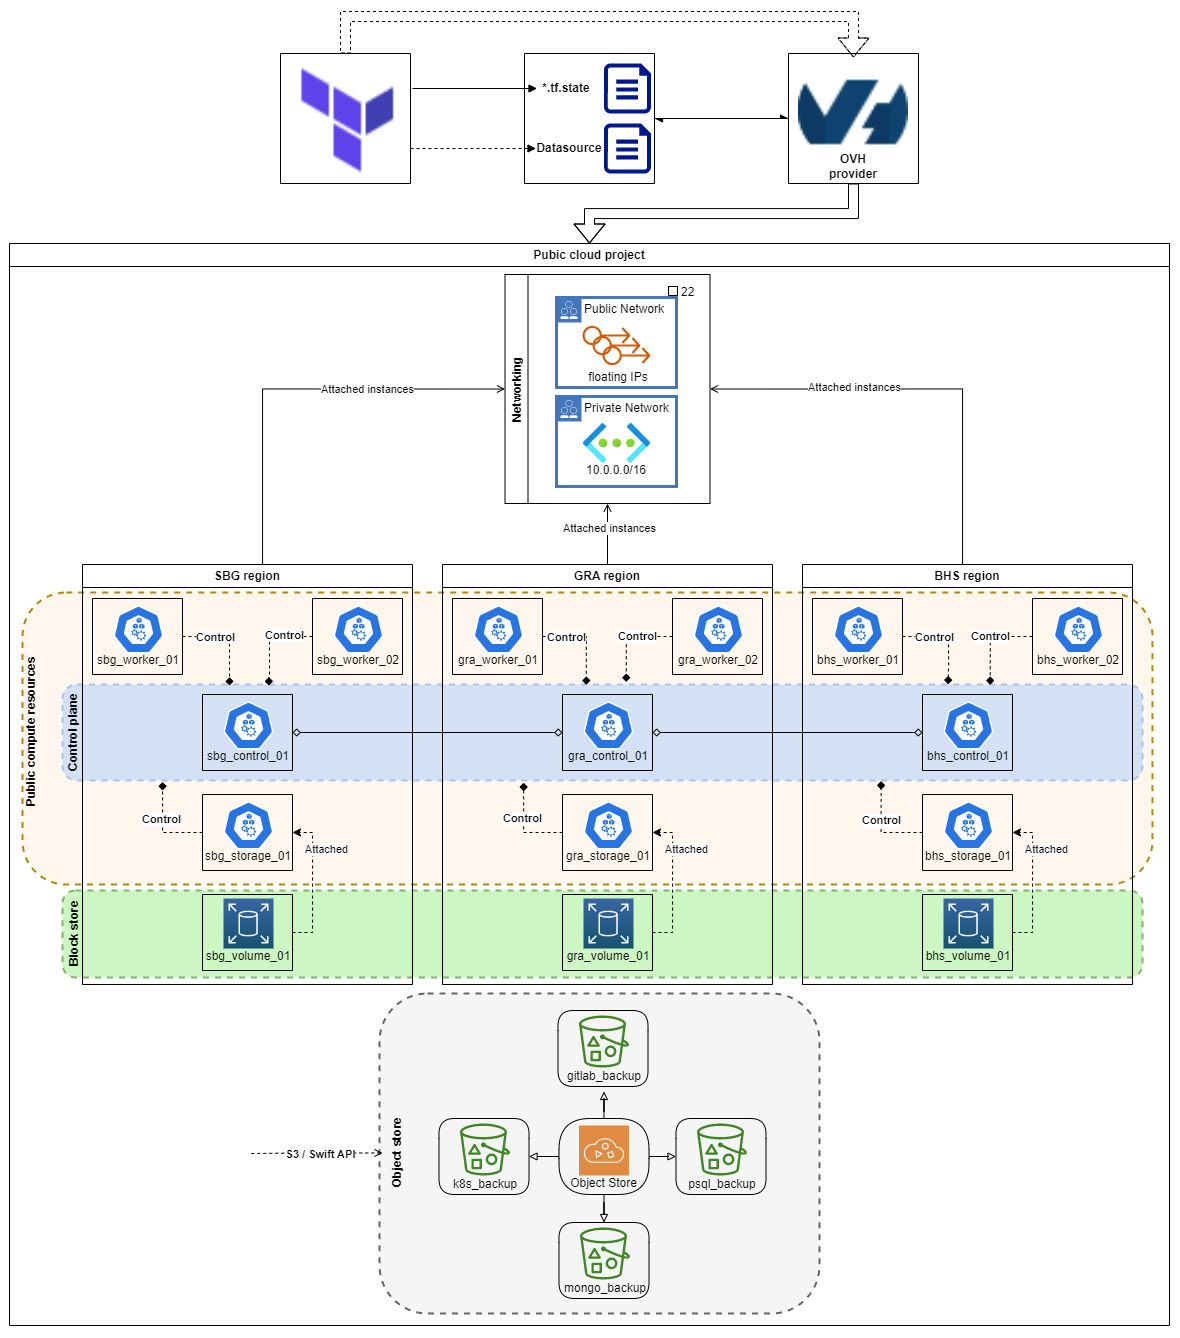
\includegraphics[width=1.0\textwidth,angle=00]{assets/f15.png}
\caption{Component diagram of provisioned resources}
\label{fig:fig15}
\end{figure}

The cluster resources were deployed to three regions. Namely, GRA, BHS, SBG. In each region, four instances were created. One of which will join the control plane, two will have the worker compute role and the last will have a second block device in raw format and will join the data storage backend. Various buckets from the object store will be provisioned and will serve as backup storage backends and high-speed data storage.
\section{Preliminary infrastructure setup}
\subsection{UML design: activity diagram for infrastructure setup}

This activity diagram illustrates how Ansible and Terraform can work together to provision infrastructure resources and set up a PaaS environment.

\begin{figure}[H]\centering
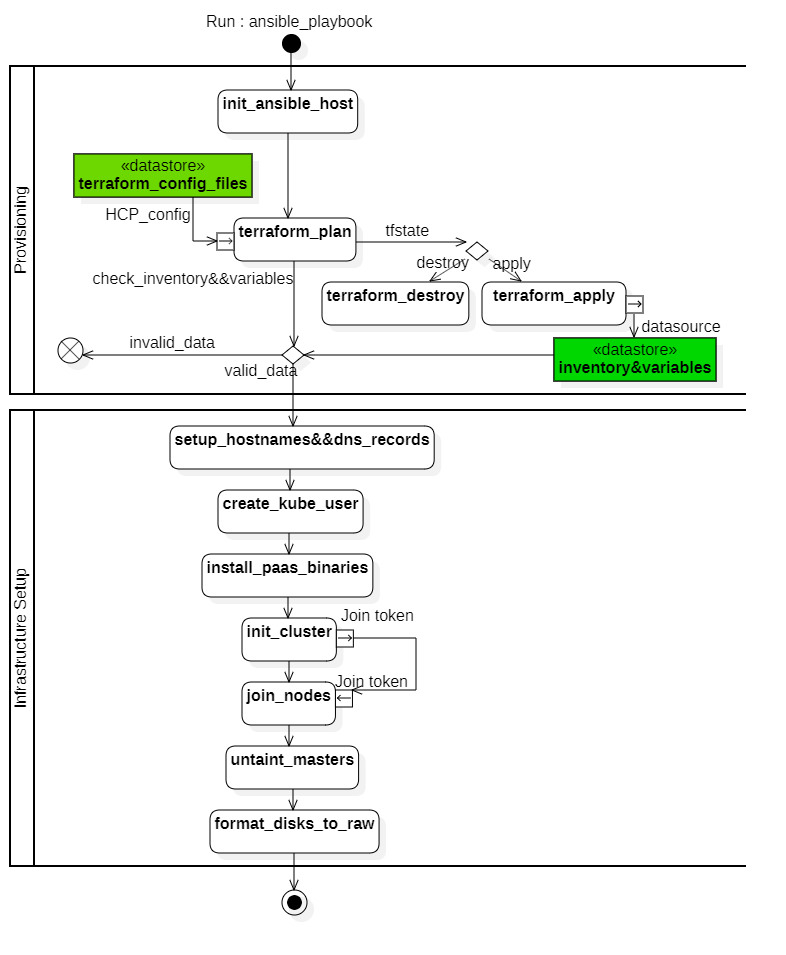
\includegraphics[width=1.0\textwidth,angle=00]{assets/f20.png}
\caption{Activity diagram for infrastructure setup}
\label{fig:activity diagram for infrastructure setup}
\end{figure}


\subsection{UML design: sequence diagram for infrastructure setup}

The following is a sequence diagram that shows the flow of actions or events that occur during the process of setting up the infrastructure.


\begin{figure}[H]\centering
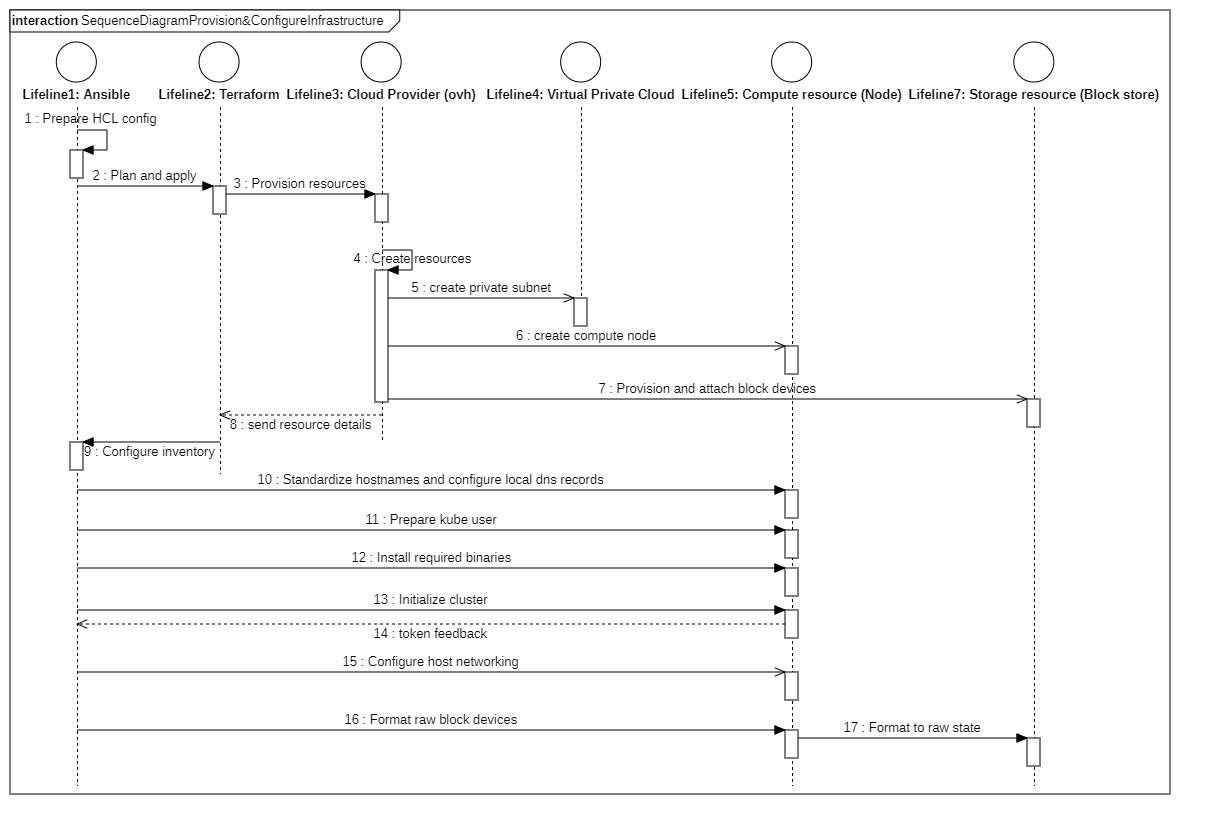
\includegraphics[width=1.0\textwidth,angle=00]{assets/f16.png}
\caption{Sequence diagram for infrastructure setup}
\label{fig:Sequence diagram for infrastructure setup}
\end{figure}

\begin{itemize}[label={--}]
    \item The user initiates the infrastructure setup process by running starting an ansible playbook.
    \item The first ansible playbook sets up the host machine to run terraform. It invokes Terraform, which then communicates with the OVH API to provision the required resources.
    \item OVH API receives the request and creates the necessary resources such as virtual machines, block storage volumes, and network interfaces.
    \item Terraform receives the response from the OVH API and applies any necessary configurations to the provisioned resources.
    \item Ansible then takes over and configures the provisioned resources by installing the required packages, setting up the network configurations, and configuring the software applications.
    \item If everything is working as expected, a notification is sent via an office 360 webhook channel. The devSecOps team is notified that the infrastructure setup process is complete, and the system is ready for use.
\end{itemize}

\subsection{Playbook diagrams for resource setup}

\subsubsection{Playbook 0: Setting up individual instances}

Next, we look at the playbook for setting up and standardizing the both the ansible host and the public cloud instances.

\begin{figure}[H]\centering
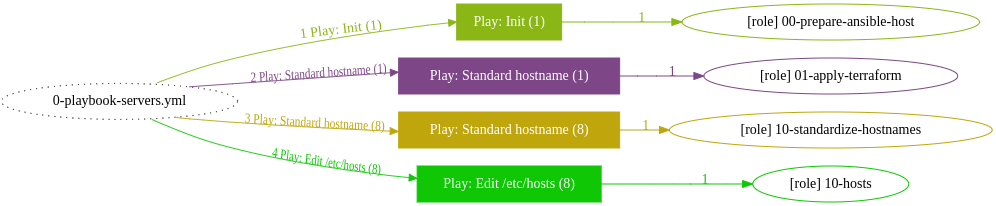
\includegraphics[width=1.0\textwidth,angle=00]{assets/f17.png}
\caption{individual instances diagram}
\label{fig:individual instances diagram}
\end{figure}

\subsubsection{Playbook 1: Orchestrated cluster setup}

For setting up the Kubernetes cluster on the provisioned infrastructure resources, the following step were automated using an ansible playbook:

\begin{itemize}[label={--}]
    \item The playbook first sets up the necessary prerequisites on each node, such as disabling swap, disabling firewall, installing necessary packages, etc.
    \item Next, it initializes the first node from the control plane as a master and joins the others as secondary masters. This involves setting up the necessary configuration files, certificates, and keys for the Kubernetes control plane.
    \item After the master node is initialized, the playbook joins the worker nodes. This involves passing the appropriate configuration information, such as the API server address and token, to the worker nodes.
    \item Once all nodes are part of the cluster, the playbook sets up networking using the CNI plugin Calico. This involves deploying the necessary network configuration files and pods to allow communication between nodes.
    \item Finally, the playbook sets up any necessary add-ons or customizations to the cluster, such as untainting master nodes, formatting block volumes to raw, adding custom scripts to switch between namespaces and contexts easily.
\end{itemize}

\begin{figure}[H]\centering
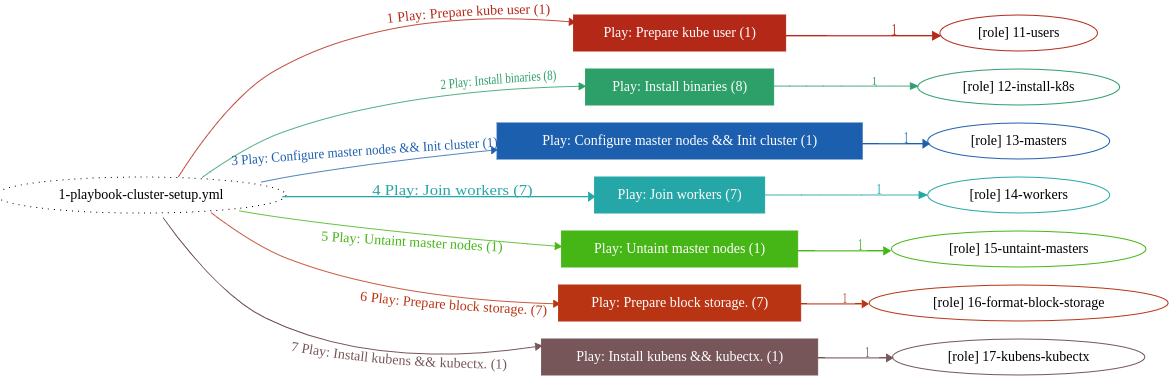
\includegraphics[width=1.0\textwidth,angle=00]{assets/f18.png}
\caption{Orchestrated cluster Diagram}
\label{fig:fig18}
\end{figure}

A summary of the previous two diagrams is depicted in the following figure :

\begin{figure}[H]\centering
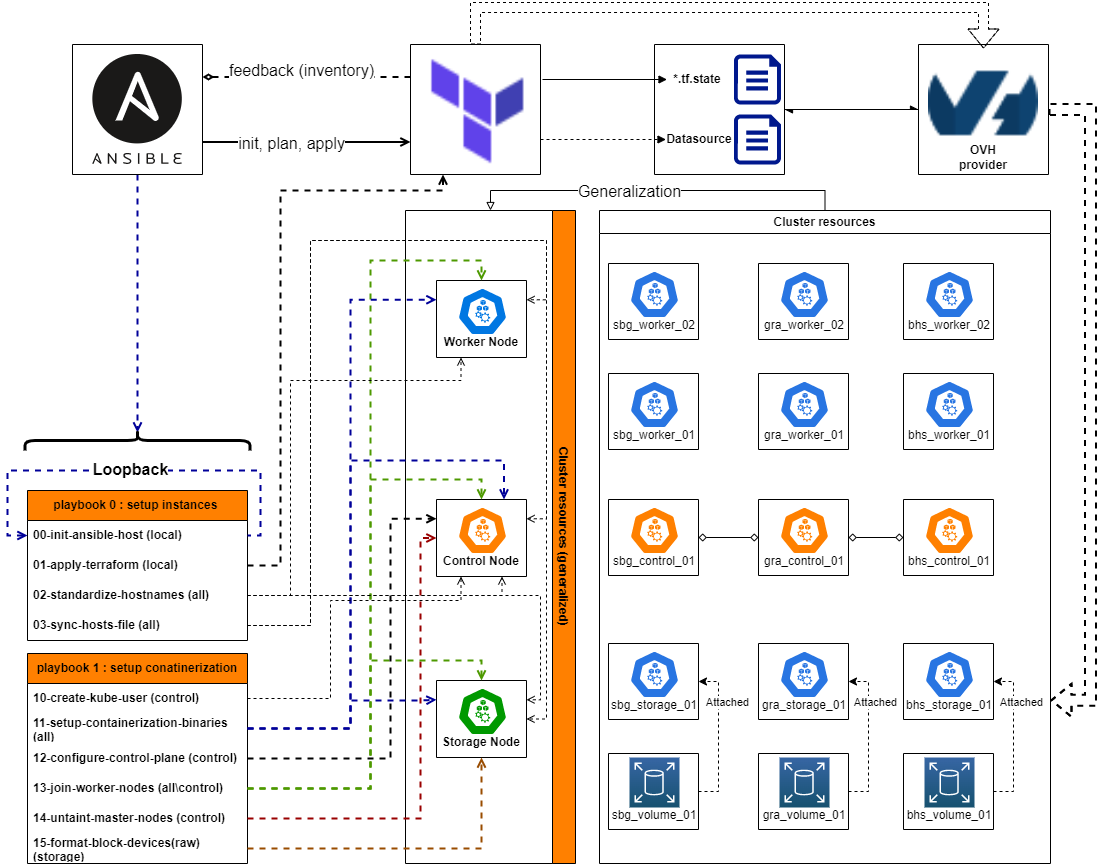
\includegraphics[width=1.0\textwidth,angle=00]{assets/f19.png}
\caption{Orchestrated cluster setup}
\label{fig:Orchestrated cluster setup}
\end{figure}
\section{Initial setup of the backen services }
\subsection{UML design: package diagram for the initial PaaS services setup}

Here, the PaaS is the main package and contains all the other packages.

Within the PaaS package, there are three sub-packages: the Kubernetes control plane, Traefik/MetalLB, and Ceph. The control plane package contains all of the components necessary for running Kubernetes (e.g., etcd, kube-proxy, etc.), while the Traefik/MetalLB package contains the Traefik and MetalLB components used for ingress and load balancing, respectively.

Finally, the Ceph package contains all of the necessary components for running distributed storage using Ceph.

\begin{figure}[H]\centering
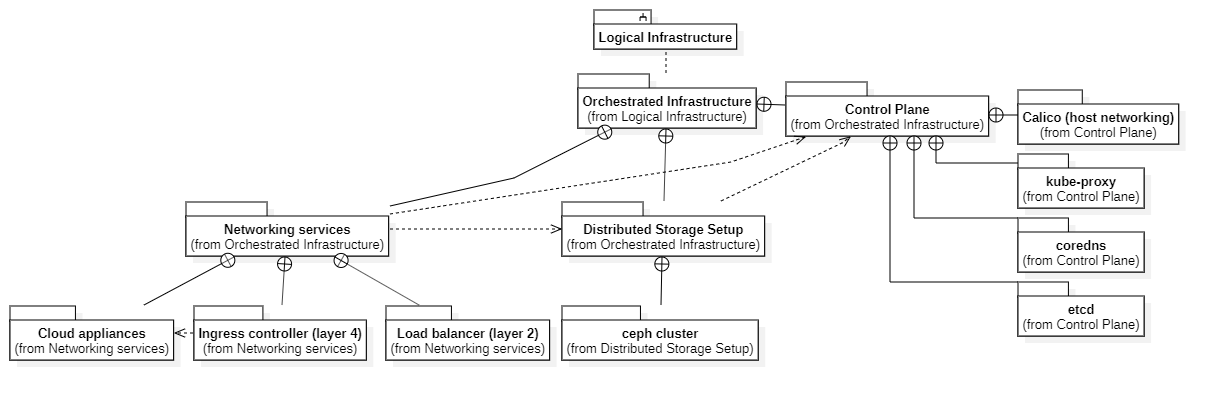
\includegraphics[width=1.0\textwidth,angle=00]{assets/f21.png}
\caption{ Package diagram for the initial PaaS setup }
\label{fig:package diagram for the initial PaaS setup}
\end{figure}

\subsection{Networking services}

\subsubsection{Overview on the networking services}

As illustrated in the following figure, Traefik, Cert-manager, and MetalLB work together to provide a secure and scalable way to route traffic inside Kubernetes using Services and IngressRoutes.

\begin{figure}[H]\centering
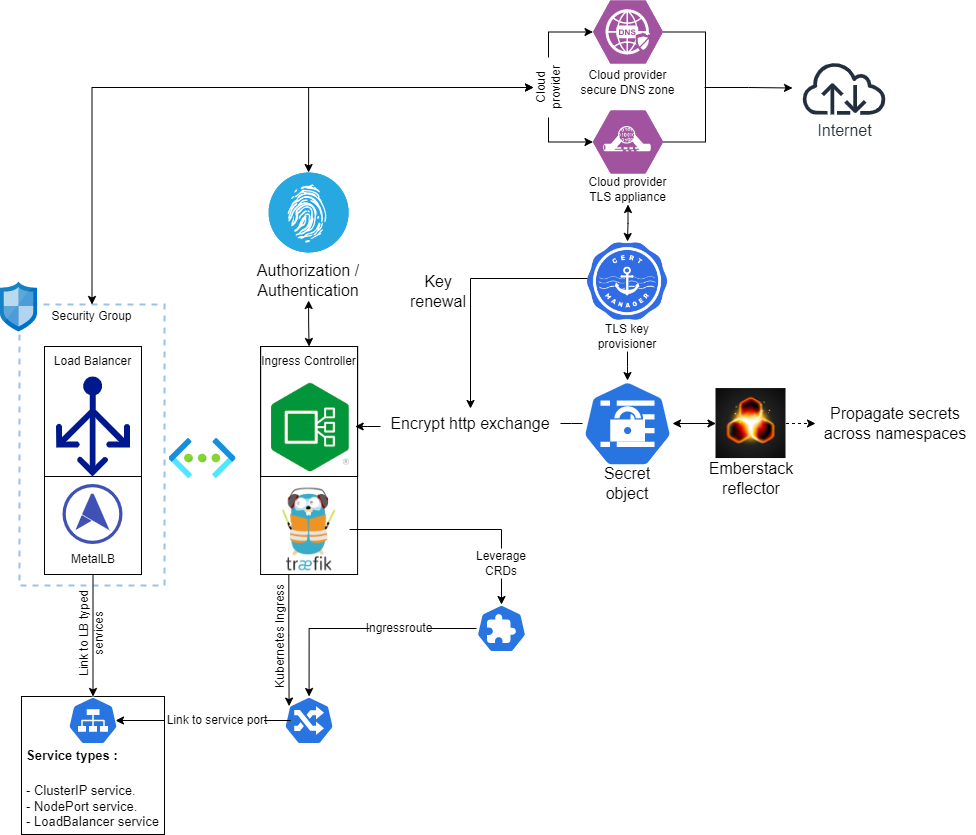
\includegraphics[width=1.0\textwidth,angle=00]{assets/f22.png}
\caption{ Networking services}
\label{fig:Networking services}
\end{figure}

Taking into consideration the following setup :
\begin{enumerate}
\item Application workloads are exposed through services of different types:
    \begin{itemize}[label={--}]
        \item ClusterIP: access from within the cluster access.
        \item LoadBalancer: access from outside the cluster using the external ip allocated through the loadbalancer.
        \item NodePort: access from outside the cluster using the ip of the node on which the application container is running.
    \end{itemize}

\item Cert-manager is configured as a cluster issuer and uses a "DNS challenge" to provision TLS certificates specific to every subdomain or domain.

\item Cert-manager listens to every declared "certificate" resource in order to process it and generate a valid "TLS certificate" that is then stored in a secret.

\item Cert-manager is configured to renew the generated certificates periodically.

\item Emberstack reflector is used to propagate secrets and configmaps across namespaces.

The flow is as follows:

\item Traffic enters from the Internet and is directed either to MetalLB for network level load balancing, or to the Traefik ingress controller for application level load balancing.

\item Traefik Proxy receives the traffic and routes it to the appropriate Kubernetes Service that is linked to a previously configured ingressroute, based on the domain name in the request.

\item The Service forwards the traffic to the appropriate Kubernetes Pod.

\item IngressRoutes are defined for workload, and Traefik uses these IngressRoutes to direct traffic to the appropriate Service.

\item Traefik is configured to use the TLS certificates generated by Cert-manager to terminate SSL/TLS traffic.

\item Traffic is routed to the correct Kubernetes Pods based on the domain name in the request.

\item The Kubernetes Pods process the requests and respond to the Traefik Proxy.

\item Traefik handles TLS termination using the secrets previously generated a
\end{enumerate}

\subsubsection{Secret provisioning and propagation:}

\subsubsubsection{TLS secret provisioning:}

In order to provide secure HTTPS communications between clients and the deployed workloads, valid TLS certificates need to be provisioned from our provider tls appliances. Our tool of choice is cert-manager.

Cert-manager provides us with a powerful and flexible way to manage TLS certificates in Kubernetes, enabling automatic provisioning and renewal of certificates from various certificate authorities, namely: "OVH Cloud Provider" and "Cloudflare".

By automating certificate management, cert-manager helps improve the security and reliability of our Kubernetes services, while reducing the operational burden of manual certificate provisioning and management.

Leveraging the capabilities of cert-manager is summarized by the following steps:

\begin{enumerate}
    \item  Having setup the stock cert-manager deployment, we first create the "ClusterIssuer" Kubernetes resource. Here we showcase a sample manifest:
        \begin{listing}[H]
        \inputminted{Yaml}{codeListing/cert_manager_cluster_issuer.yml}
        \caption{Cert manager cluster issuer}
        \label{lst:the-code}
        \end{listing}
    The cluster issuer manifest contains the credentials cert-manager uses to authenticate with our domain registrar (OVH). It needs these credentials to perform a DNS-01 challenge mechanism to validate domain ownership and issue TLS certificates.
    \item Next, for every domain or subdomain a "Certificate" resource is created. This certificate resource is then processed by cert-manager and results in a secret containing a TLS certificate. The following is a certificate declaration for wildcard subdomain:

\end{enumerate}
\begin{listing}[H]
\inputminted{Yaml}{codeListing/cert_manager_certificate.yml}
\caption{Cert manager certificate }
\label{lst:certificate}
\end{listing}
\subsubsubsection{Secret propagation}

Emberstack Reflector, an open-source tool that provides a simple and efficient way to propagate Kubernetes secrets across multiple namespaces and clusters. We are using it to automatically replicate a secret from a source namespace to one or more targets, ensuring that all applications that require access to the secret can access it easily.

Having deployed this tool, adding the following annotation to any secret or configmap will replicate it to every namespace:


\subsubsection{Layer 7 load balancing: application level }

Traefik, our ingress controller of choice, functions both as a reverse proxy as well as a load balancer for the deployed workload which are then accessed through secure HTTPS. 

In the following section we provide, in detail, how traefik is plugged into the cluster and how it is leveraged: 

- Deploy traefik as a "DaemonSet". Deploying traefik as a daemonset allows us to spawn instances of it in every node and thus take full advantage of the internet bandwidth since the workload is distributed across all cluster instances. The following Kubernetes resources are created in order to setup it up:

\begin{enumerate}
\item traefik\_rbac.yml: defines Roles and RoleBindings to grant users or groups specific permissions for accessing Traefik's API and resources.
\item traefik\_crds.yml: allow us to extend the Kubernetes API and define custom resources that enable more advanced features and configuration options such as "IngressRoutes" for services, "TLSStores", "Middlewares", etc.
\item traefik\_service\_account.yml:  
\item traefik\_pvc.yml:  a persistent volume claim that resolves to a volumes which then will be attached to pods to persist the storage of data. 
\item traefik\_daemonset.yml: the actual deployment for traefik. It spawns an instance of traefik in every node of the cluster. 
\item traefik\_ingressclass.yml: the IngressClass resource that specifies which Traefik instance should handle requests for a particular Ingress. 
\item traefik\_tls\_store.yml: a configuration object that enables us to store and manage TLS certificates and keys for use in TLS termination, encryption, and authentication. 
\item traefik\_dashboard\_ingressroute.yml: a Kubernetes Custom Resource Definition (CRD) that allows us to define advanced routing rules and configurations for Traefik. They are similar to Kubernetes Ingress resources but provide additional functionality and flexibility. 
\end{enumerate}

Note that traefik is capable of receiving configurations from the built-in Kubernetes ingress resource. 

Here we have the dashboard of traefik: 

\begin{figure}[H]\centering
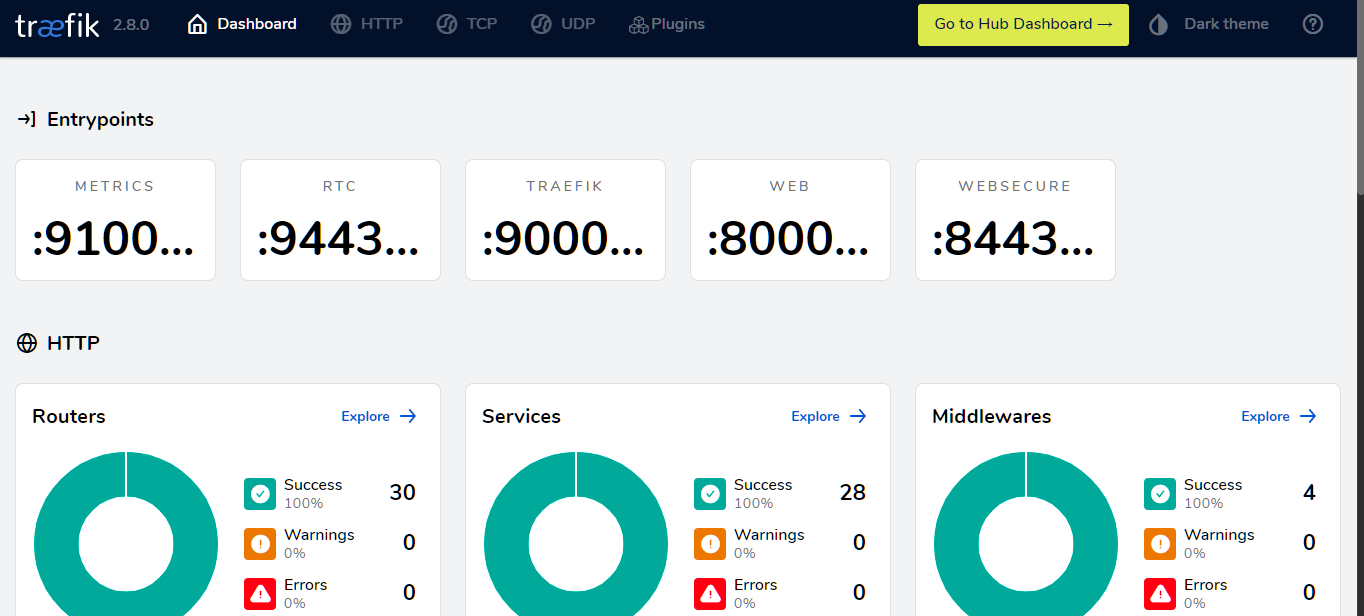
\includegraphics[width=1.0\textwidth,angle=00]{assets/f25.png}
\caption{ Dashboard of traefik }
\label{fig:dashboard of traefik}
\end{figure}

Notice that traefik has multiple entrypoints configured depending on the protocol and the use case. The main entrypoint is websecure. It regulates the HTTPS traffic.  

When Traefik receives an incoming request, it can use the TLS Store to look up the appropriate certificate for the requested domain and use it to encrypt and decrypt traffic. 

Traefik is used in combination with the security layer services to allow for authenticating and authorizing access. The security layer will be discussed in detail further in this report. 

\subsubsection{Layer 4 load balancing: network level }

In this level, load balancing is mostly related to the network, IP addresses, network address translation ( NAT ), and packets. 

\begin{enumerate}[label = (\alph*)]

\item Using the built in Kubernetes capability : NodePort services 
The NodePort Service exposes a deployment or a set of pods by mapping a specific port on each node in the cluster to the port of the service. 
This allows external clients to access the service by connecting to any of the nodes in the cluster. 
Here's how NodePort Services work: 
    \begin{enumerate}[label = (\arabic*)]
    \item A NodePort Service is defined as a Kubernetes object with the           "type: NodePort" field in the YAML manifest. 
    \item When a NodePort Service is created, Kubernetes assigns a high port number (in the range 30000-32767) to the service. 
    \item Kubernetes then maps the assigned port to the port of the service, which can be any valid port number. 
    \item The NodePort Service is then exposed on all nodes in the cluster, allowing external clients to access the service by connecting to any of the nodes on the assigned port. 
    \item Traffic received on the assigned port is forwarded to the service's target port, which is the port on which the service is listening. 
    \item Kubernetes ensures that the traffic is load balanced across all pods that are part of the service. 
    \end{enumerate}

\item Using metalLB for load balancing : LoadBalancer services 
MetalLB is used to provide network load balancing for services running in the cluster. Here's how MetalLB works in our Kubernetes cluster: 

    \begin{itemize}[label={--}]
        \item MetalLB is deployed in the cluster using the following manifests: 
            \begin{enumerate}[label = (\arabic*)]
            \item "metalLB\_configmap.yml": a configmap resource containing the ip address pool that metalLB is allowed to use to allocate to loadbalancer-type services. As a sample, here is the code snippet for this configmap, the rest will be added in the index section of this document : 

            \begin{listing}
            \inputminted{Yaml}{codeListing/metalLB_configmap.yml}
            \caption{Cert manager certificate }
            \label{lst:metalLB}
            \end{listing}

            \item "metalLB\_rbac.yml": a method of providing fine-grained access control in Kubernetes. RBAC is a security mechanism that restricts access to resources and operations based on the roles assigned to users or service accounts in the cluster. 
            \item "metalLB\_service\_account.yml": an identity that is used by a pod or a set of pods to access the Kubernetes API server and other resources in the cluster. 
            \item "metalLB\_controller.yml": a deployment that watches for changes to load balancer services in the cluster and dynamically assigns IP addresses to those services as needed. 
            \item "metalLB\_speaker.yml": a daemonset that spawns a pod in every node in the cluster it is responsible for announcing the allocated IP addresses for load balancer services. 
            \item "metalLB\_pod\_security\_policy.yml": It allows the definition of a set of security policies that pods must comply with to be scheduled and run on nodes in the cluster. In the context of MetalLB, this PSP is used to enforce security measures for the MetalLB components, including the MetalLB controller and the MetalLB speaker. 
            \end{enumerate}

        \item Exposing a workload using the deployed metalLB loadbalancer is as follows: 
            \begin{enumerate}[label = (\arabic*)]
                \item After creating the application deployment, we create a Kubernetes Service that exposes this workload using the "type" field of the Service to "LoadBalancer". 
                \item Once the Service is created, MetalLB will allocate an IP address from the configured pool of addresses and assign it to the Service. 
                \item We then use this IP address to access your workload from outside the cluster. 
            \end{enumerate}
        \item This is a sample service of the "LoadBalancer" type: 
        
        \begin{figure}[H]\centering
        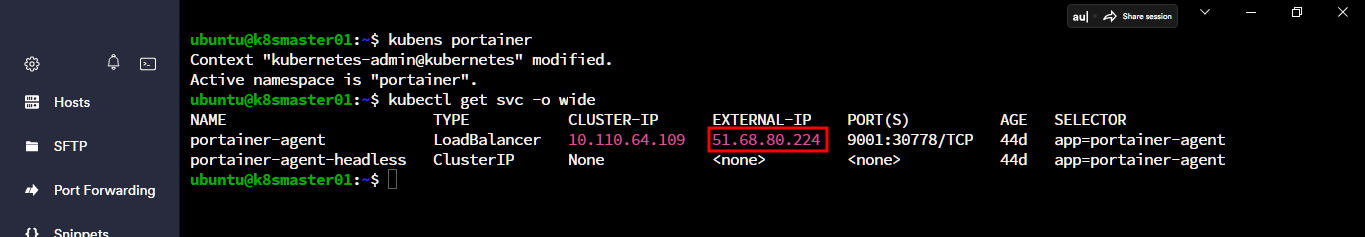
\includegraphics[width=1.0\textwidth,angle=00]{assets/f23.png}
        \caption{LoadBalancer service }
        \label{fig:LoadBalancer}
        \end{figure}
        
    \end{itemize}

\end{enumerate}

\subsection{Distributed storage backend}

\subsubsection{Architectural overview on storage}

Distributed persistent storage is important for running stateful applications such as databases that require durable storage. In our context, the ability to store data persistently across multiple nodes in a cluster is implemented using the following architecture: 

\begin{figure}[H]\centering
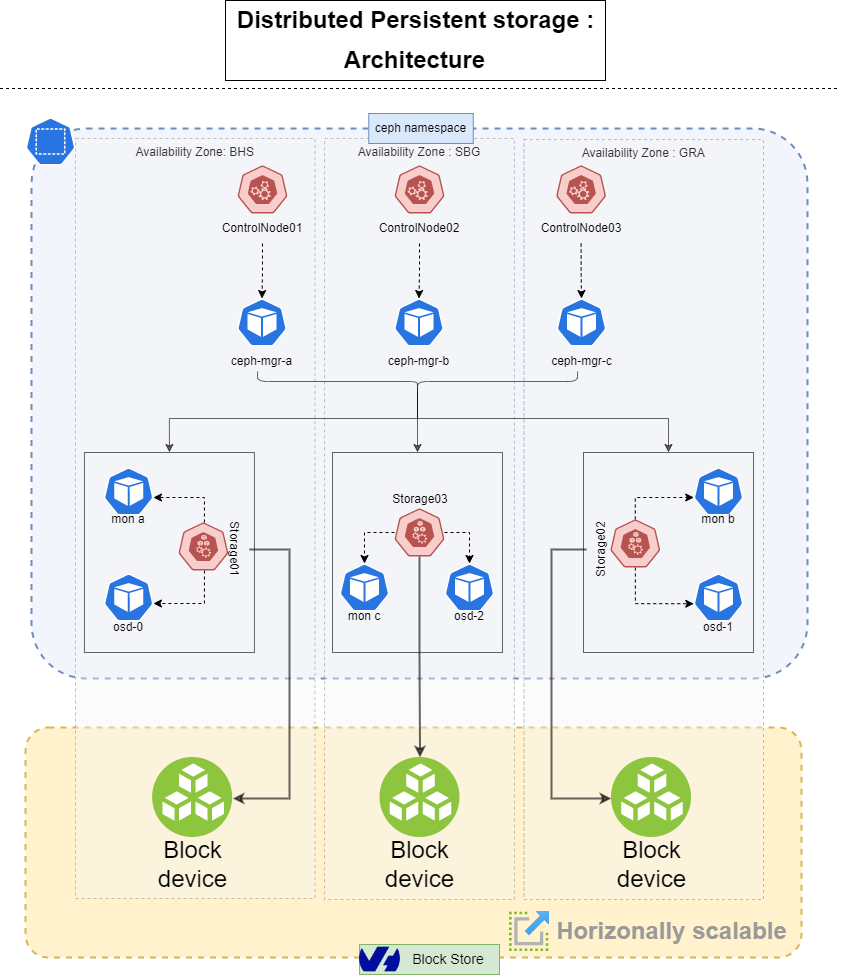
\includegraphics[width=1.0\textwidth,angle=00]{assets/f26.png}
\caption{Architectural overview on storage}
\label{fig:Architectural overview on storage}
\end{figure}

The figure above illustrates a highly scalable storage architecture using “Ceph”. As mentioned in the infrastructure provisioning chapter, in each region, we have created a dedicated storage instance to which a disk the raw format has been attached. The number of disks attached to each node is infinitely scalable and only dependent on the specs of the instance to which it is attached. Furthermore, the size of each disk can be scaled up by the cloud provider. That being said, the number of instances is itself theoretically infinitely scalable. And thus, both horizontal and vertical scalability is achieved. 

\subsubsection{Ceph as a storage provider for kubernetes }

“Ceph”, our storage provider is deployed as a resource. It includes several components, such as the Ceph monitor, manager, OSD (object storage daemon), and MDS (metadata server), that work together to provide distributed storage: 

\begin{itemize}[label={--}]
    \item First, we deploy the operator, which is a Kubernetes-native controller that automates the deployment and management of the Ceph storage cluster. 
    \begin{figure}[H]\centering
    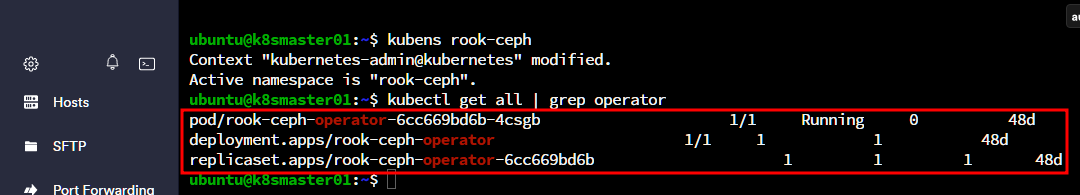
\includegraphics[width=1.0\textwidth,angle=00]{assets/f27.png}
    % \caption{Figure 27 }
    % \label{fig:f27}
    \end{figure}
    \item Next we create a CephCluster custom resource, which defines the desired state of the Ceph cluster.
    \begin{figure}[H]\centering
    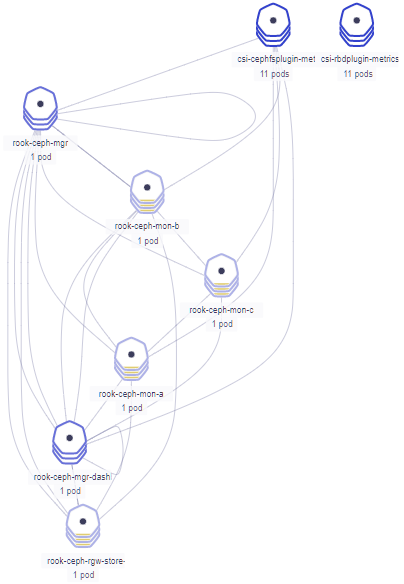
\includegraphics[width=1.0\textwidth,angle=00]{assets/f28.png}
    % \caption{Figure 28 }
    % \label{fig:f28}
    \end{figure}
    \end{itemize}
Ceph is configured such that it will use every raw block device attached to the storage nodes to join it to its storage pool. For each storageNode, the operator spawns an OSD (Object Storage Daemon) which is a storage node that stores objects, e.g., the basic units of data.  
Using the ingress controller, a dashboard for “ceph” is exposed and allows for observability on the storage backend: 
\begin{figure}[H]\centering
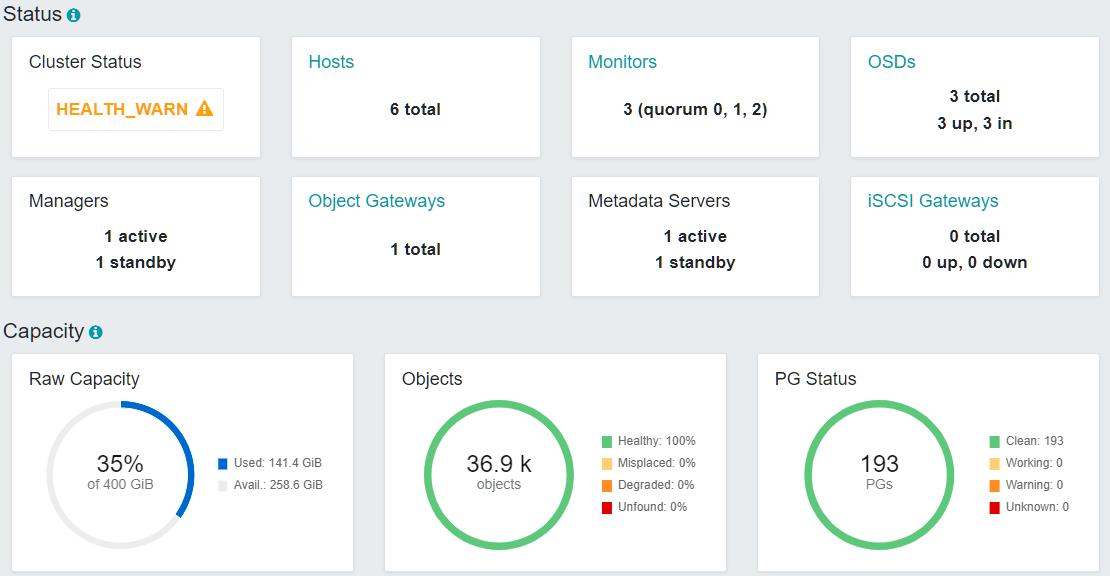
\includegraphics[width=1.0\textwidth,angle=00]{assets/f29.png}
\caption{Ceph Dashboard }
\label{fig:Ceph Dashboard }
\end{figure}

\subsubsection{Deployed storage capabilities: }

The following diagram provides an overview on the storage capabilities of ceph : 
\begin{figure}[H]\centering
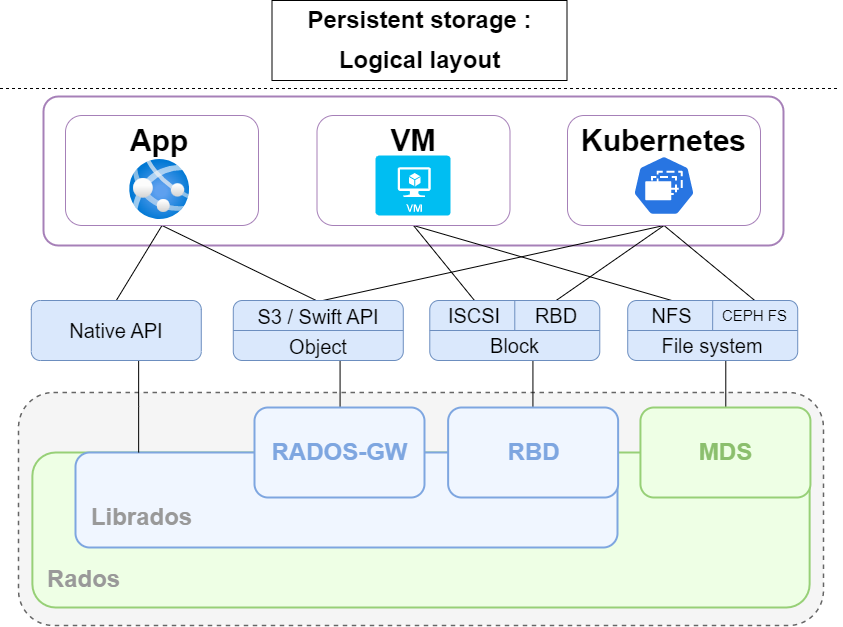
\includegraphics[width=1.0\textwidth,angle=00]{assets/f30.png}
\caption{Storage capabilities Diagram}
\label{fig:f30}
\end{figure}

\subsubsubsection{Filesystem storage mode: }

CephFS works by creating a virtual file system on top of the RADOS object store, which allows multiple clients to access the same file system concurrently. 

In order to leverage the filesystem storage mode in the service of the deployed workloads in the cluster: 
\begin{enumerate}[label = (\arabic*)]
    \item A CephFilesystem CRD is created. 
    \item Next, a StorageClass that specifies the storage parameters for the file system, such as the size of the file system and the type of file system (e.g., ext4 or xfs). 
    \item A Persistent Volume Claim is created. 
    \item When a pod requests a volume that matches the PVC, Kubernetes (the CSI provisioner) will dynamically provision a volume from the CephFS file system and mount it to the pod. 
\end{enumerate}
As shown by the figure below, CephFS provides built-in redundancy and fault tolerance, ensuring that data is always available even in the event of hardware failures. 
\begin{figure}[H]\centering
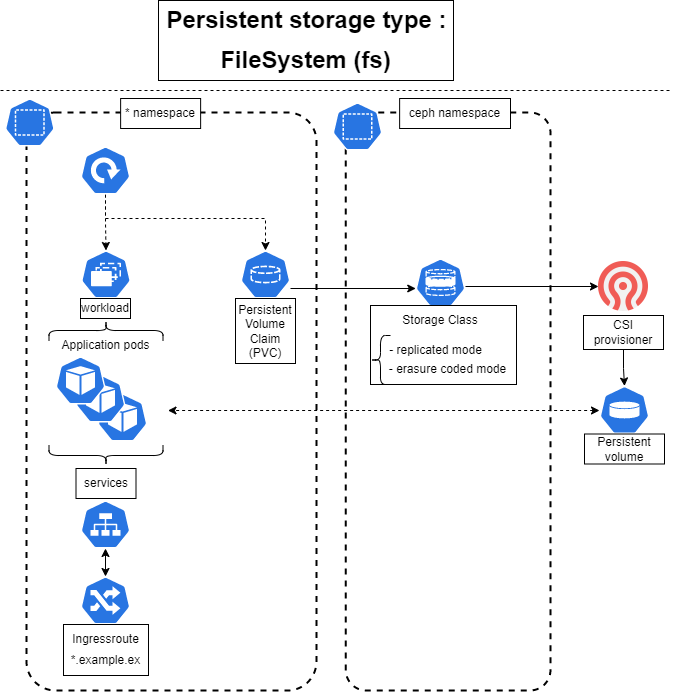
\includegraphics[width=1.0\textwidth,angle=00]{assets/f31.png}
\caption{Filesystem Storage}
\label{fig:Filesystem Storage}
\end{figure}

\subsubsubsection{Object storage mode: }

It stores data as objects, rather than as files or blocks. This allows applications to store and retrieve large amounts of unstructured data in a highly available and fault-tolerant manner. 

Ceph Object Storage exposes an S3-compatible API. 

The procedure to provision object store buckets is as follows: 

\begin{enumerate}[label = (\arabic*)]
    \item First we create the CephObjectStore CRD that starts the RGW (RadosGateWay) service in the cluster with an S3 API. 
    \item Next, an object store StorageClass is created. It contains such as the reclaimPolicy and the objectStore to which it is linked. 
    \item Finally, for every bucket we desire to create, we either use the S3 API to converse with the RGW or we declare an ObjectBucketClaim which will then be resolved to a bucket. 
\end{enumerate}


This procedure is summarized by the following figure: 

\begin{figure}[H]\centering
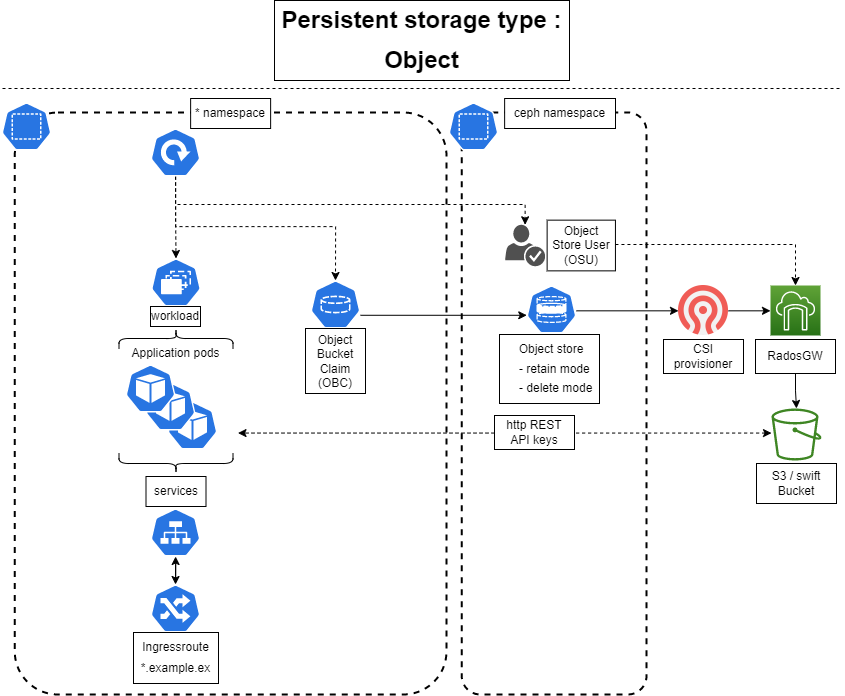
\includegraphics[width=1.0\textwidth,angle=00]{assets/f32.png}
\caption{Object Storage mode }
\label{fig:Object Storage mode}
\end{figure}

\subsubsubsection{Block storage mode: }

Ceph Block Storage exposes a block device interface. But due to the very nature of a containerized environment, we are not using this capability. The following is a summary on the procedure to provision block devices using ceph: 

\begin{figure}[H]\centering
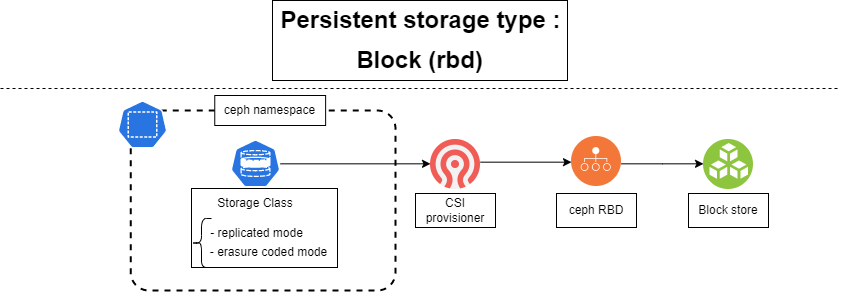
\includegraphics[width=1.0\textwidth,angle=00]{assets/f33.png}
\caption{Block Storage Procedure}
\label{fig:Block Storage Procedure}
\end{figure}

The following are the basic steps involved: 

\begin{enumerate}[label = (\arabic*)]
\item Create the CephBlockPool CRD : defines a specific type of Ceph storage pool. It is used to provision block storage volumes on a Ceph cluster for Kubernetes applications. It specifies a Ceph storage pool with certain parameters, such as the number of replicas, disk size, and disk type. 
\item Create the StorageClass: a Kubernetes StorageClass that references the Ceph cluster. This StorageClass defines the properties of the block storage volumes that will be created, such as the replication factor and the type of storage pool. 
\item Create the PersistentVolumeClaim (PVC): Once the StorageClass is created, we create a PersistentVolumeClaim (PVC) using the StorageClass. This PVC requests a block storage volume of a certain size and other properties defined in the StorageClass. 
\item Attach PVC to Pod: Finally, we attach the PVC to a Kubernetes Pod as a volume. This allows the Pod to use the block storage volume as a local disk. 
\end{enumerate}

When a Pod is created, Kubernetes automatically provisions a block storage volume by creating a block device in the Ceph cluster and attaching it to the Pod. 

When the Pod is deleted, the block storage volume is automatically deleted as well. This is contingent on the parameter “reclaimPolicy: Delete” in the storage class. Otherwise, we define a storage class with the parameter “reclaimPolicy: retain”. 

This provides dynamic and on-demand provisioning of block storage volumes to the applications running on Kubernetes.

\section{Authentication and authorization}
\subsection{Conceptual overview }

Previously, traefik has been deployed and configured to serve as an ingress controller and load balancer for our platform as a service. In this chapter we discuss how an assortment of components are used in combination with traefik to provide a secure and scalable solution for authentication and authorization. 

The following diagram illustrates the layout of this architecture: 

\begin{figure}[H]\centering
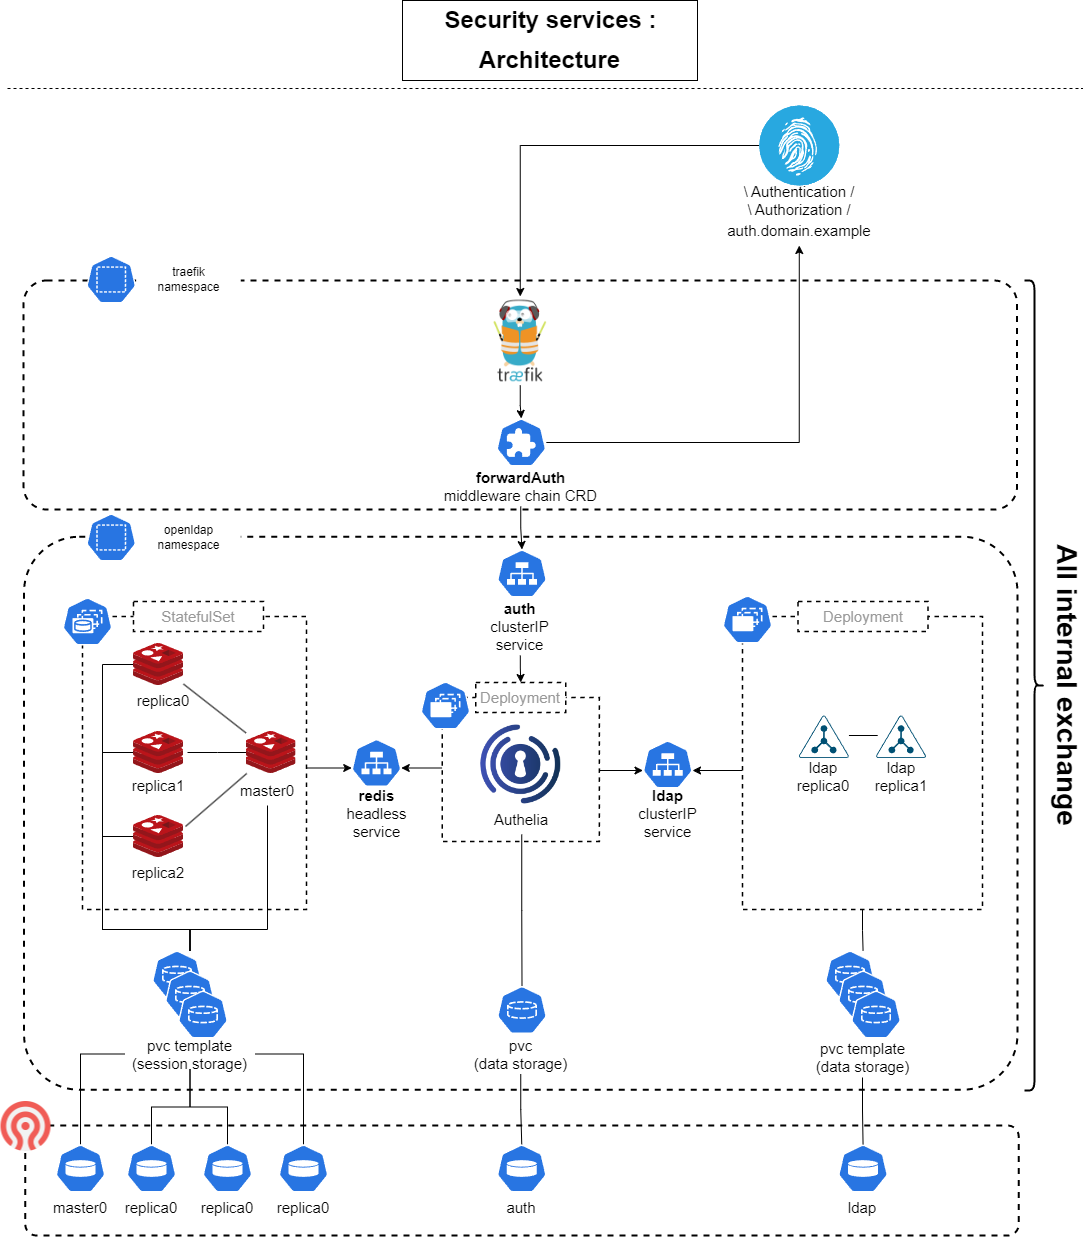
\includegraphics[width=1.0\textwidth,angle=00]{assets/f51.png}
\caption{Conceptual overview }
\label{fig:f51}
\end{figure}

\textbf{Traefik} is used as a reverse proxy and ingress controller, which allows external traffic to access the applications running inside the Kubernetes cluster. Traefik provides load balancing, SSL termination, and routing based on rules defined in its configuration. 

\textbf{Authelia} is used as a forward authentication and authorization controller, which provides an additional layer of security by enforcing authentication and authorization before requests are forwarded to the backend services. Authelia also provides Single Sign-On (SSO) functionality, allowing users to authenticate once and access multiple applications seamlessly. 

\textbf{OpenLDAP}, which stores user information and credentials for authentication and authorization purposes, is used as an LDAP server in conjunction with a web interface to facilitate management. 

Authelia authenticates users against the OpenLDAP server and authorizes access to resources based on LDAP group membership. 

\textbf{Redis} is used for session storage, which stores user session information to ensure that users remain authenticated and authorized throughout their session. 

 

\subsection{Deployment and configuration of components }

\subsubsection{openLDAP for access and user management  }

A custom openldap server is deployed for the purpose of safely and reliably accessing and managing the distributed directories that store information about users, groups, resources. 

\subsubsubsection{Deployment: }

An ansible playbook is firstly run to perform the following steps : 
\begin{itemize}[label={--}]
\item Using the “community.docker.docker\_image” library, building the custom container image of the openLDAP server as well as the web interface. 
\item Using the “community.docker.docker\_image” library, pushings the built images to the private registry. 
\item Using the “kubernetes.core.k8s” library, applying the manifests to deploy the server. 
\end{itemize}

The following is a code snippet from the manifest for deploying the openLDAP server: 

\begin{listing}[H]
\inputminted[firstline=1,lastline=10]{Yaml}{codeListing/deploy_openldap.yml}
\end{listing} 

\begin{listing}[H]
\inputminted[firstline=16,lastline=55]{Yaml}{codeListing/deploy_openldap.yml}
\end{listing} 

\begin{listing}[H]
\inputminted[firstline=56]{Yaml}{codeListing/deploy_openldap.yml}
\caption{Deploying openLDAP}
\label{lst:Deploying_openLDAP}
\end{listing} 

\subsubsubsection{Resource overview }

The web interface below is deployed and configured to provide secure remote access to the openLDAP server entries, thus allowing management operations. This is achieved using the LDAP base name of the company. Naturally, external direct access to server is prohibited. 
\begin{figure}[H]\centering
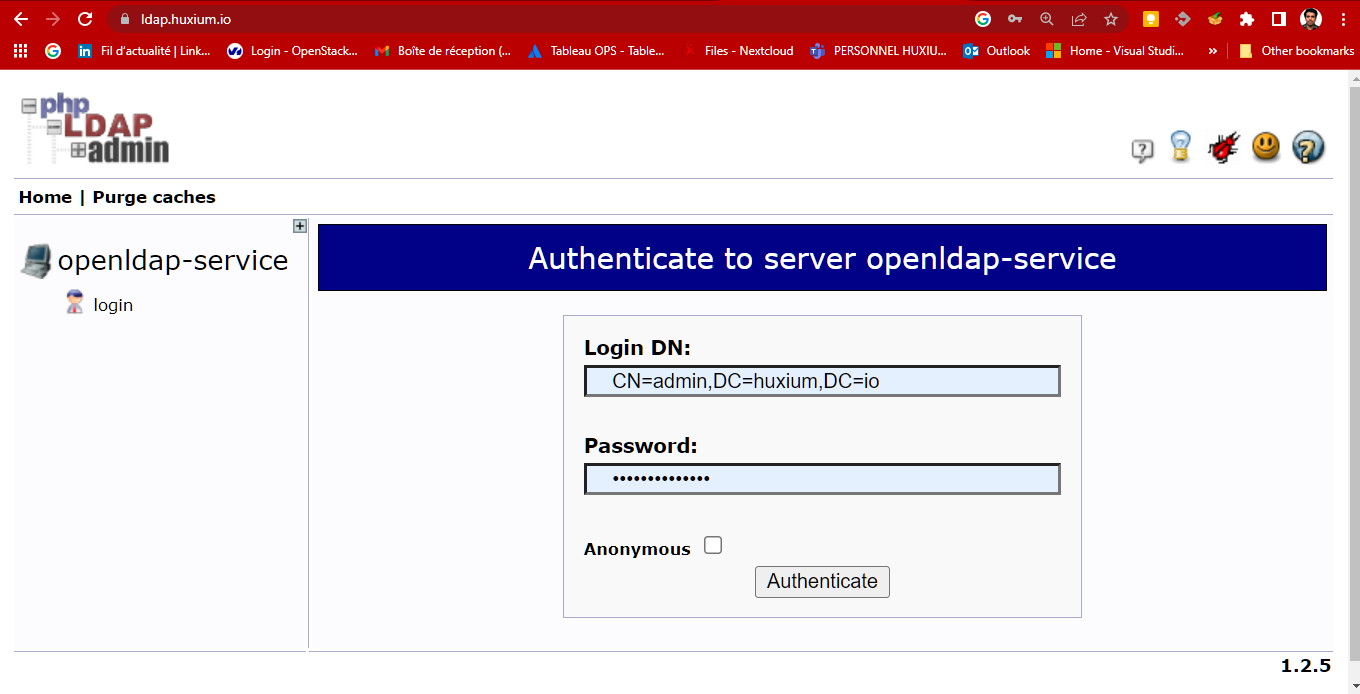
\includegraphics[width=1.0\textwidth,angle=00]{assets/f52.png}
\caption{Figure 52 }
\label{fig:f52}
\end{figure} 

\subsubsection{Redis for session storage }

Redis is used with the “auth-middleware” for session storage because Redis is an efficient and highly scalable in-memory data store that can handle high-traffic web applications. 

\subsubsubsection{Deployment:} 

When users log in, their authentication and session data are stored in a session cookie, which is used to authenticate them on subsequent requests. 

By using Redis as the session store for Authelia, it becomes possible to store these session cookies in a highly available and scalable data store that can be shared across multiple Authelia instances.  

This is important for applications that experience heavy traffic, as it ensures that user authentication data can be retrieved and verified quickly and efficiently. 

\subsubsubsection{Resource overview: }

The following is an overview of the resulting ReplicaSet for Redis: 

\begin{figure}[H]\centering
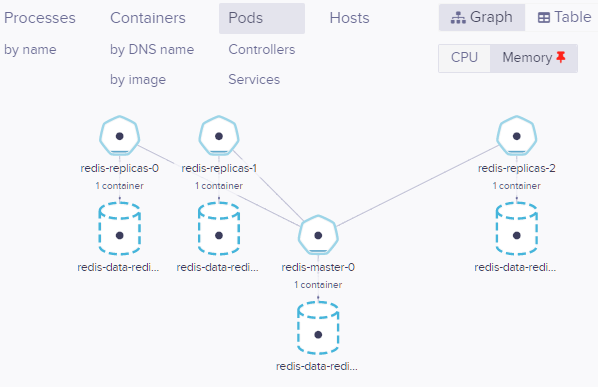
\includegraphics[width=1.0\textwidth,angle=00]{assets/f53.png}
\caption{Figure 53 }
\label{fig:f53}
\end{figure}

The ReplicaSet contains 4 pods with a persistent volume each. The pod hierarchy is as follows: 
\begin{itemize}[label={--}]
\item One master pod with the read/write privilege. 
\item Three replicas with read-only access. 
\end{itemize}
Only internal access is allowed. This is achieved using the following services: 

\begin{itemize}[label={--}]
\item redis-master.openldap.svc.cluster.local for read/write operations (port 6379) 
\item redis-replicas.openldap.svc.cluster.local for read-only operations (port 6379) 
\end{itemize}



\subsubsection{Authelia for single sign-on }

Authelia is put in place to provide a single sign-on experience and fine-grained access control for applications and services running on the cluster.  

\subsubsubsection{Deployment: }

It leverages the LDAP server to cross-check user credentials. Two backend database servers are configured. Authelia uses the HA PostgreSQL cluster to store policies and other data. It also relies on the replicated Redis cluster for user session storage. 

The following configuration is attached to the authelia containers using the configmap binding method: 

\begin{listing}[H]
    \inputminted[firstline=1,lastline=25]{Yaml}{codeListing/authelia_configmap.yml}
\end{listing}

\begin{listing}[H]
    \inputminted[firstline=26,lastline=55]{Yaml}{codeListing/authelia_configmap.yml}
\end{listing}

\begin{listing}[H]
    \inputminted[firstline=56]{Yaml}{codeListing/authelia_configmap.yml}
    \caption{Authelia configuration}
    \label{lst:Authelia configuration}
\end{listing}

\subsubsubsection{Resource overview : }

The following is an overview of the deployed resources: 
\begin{figure}[H]\centering
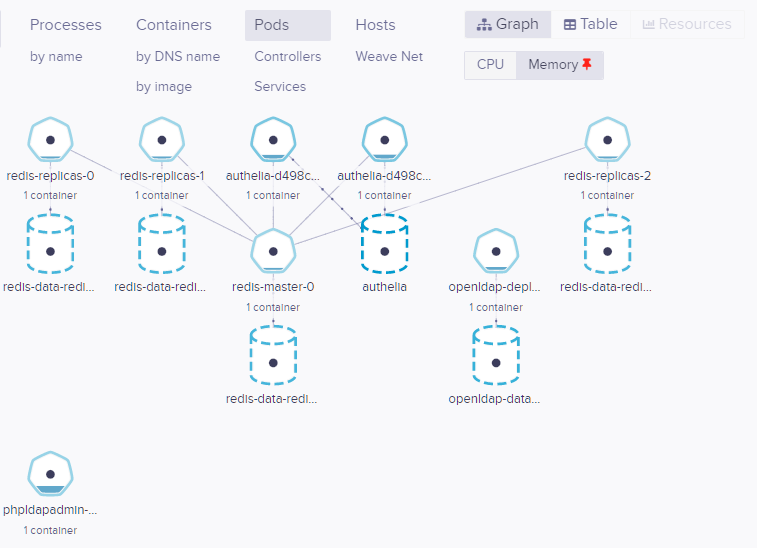
\includegraphics[width=1.0\textwidth,angle=00]{assets/f54.png}
\caption{Deployed resources}
\label{fig:f54}
\end{figure}


This diagram features the following elements: 

\begin{itemize}[label={--}]
\item A deployment of authelia configured with a horizontal pod autoscaler.  
\item The replicated Redis cluster to stora session data. 
\item The openLDAP server that houses user credentials. 
\end{itemize}

Each of these workloads has volumes attached to it in order to persist data. 

\subsection{The authentication gateway in action }

\subsubsection{Preliminary configuration }

As a first step, the “Middleware CRDs” that handle the request forwarding is configured. 

Naturally, communication between the ingress controller, Traefik, and the authentication server, Authelia, is exchanged internally in the cluster. 

\subsubsubsection{The “forward-auth” middleware }

Forward authentication with Traefik means that incoming requests to a service are first authenticated by the authentication server, Authelia, before being forwarded to the service. 

The following is the code snippet of this declaration: 

\begin{listing}[H]
    \inputminted{Yaml}{codeListing/middleware_forward_auth.yml}
    \caption{forward-auth middleware}
    \label{lst:forward-auth middleware}
\end{listing}

The “headers” middleware 

The “headers” middleware is a collection of middleware components that are used to authenticate and authorize HTTP requests based on various headers.  

\begin{listing}[H]
    \inputminted{Yaml}{codeListing/middleware_headers.yml}
    \caption{headers middleware}
    \label{lst:headers middleware}
\end{listing} 

These headers can include the Authorization header, session cookies, and other custom headers that contain authentication information. 

\subsubsection{Implementation }

\subsubsubsection{The authentication portal }

A chain of the “Middleware CRDs” declared above is leveraged in the following  ingressroute to deploy the authentication portal: 

\begin{listing}[H]
\inputminted{Yaml}{codeListing/authelia_ingressroute.yml}
\caption{authelia ingressroute}
\label{lst:authelia ingressroute}
\end{listing}

The following figure shows the authentication portal as seen by an external user: 
\begin{figure}[H]\centering
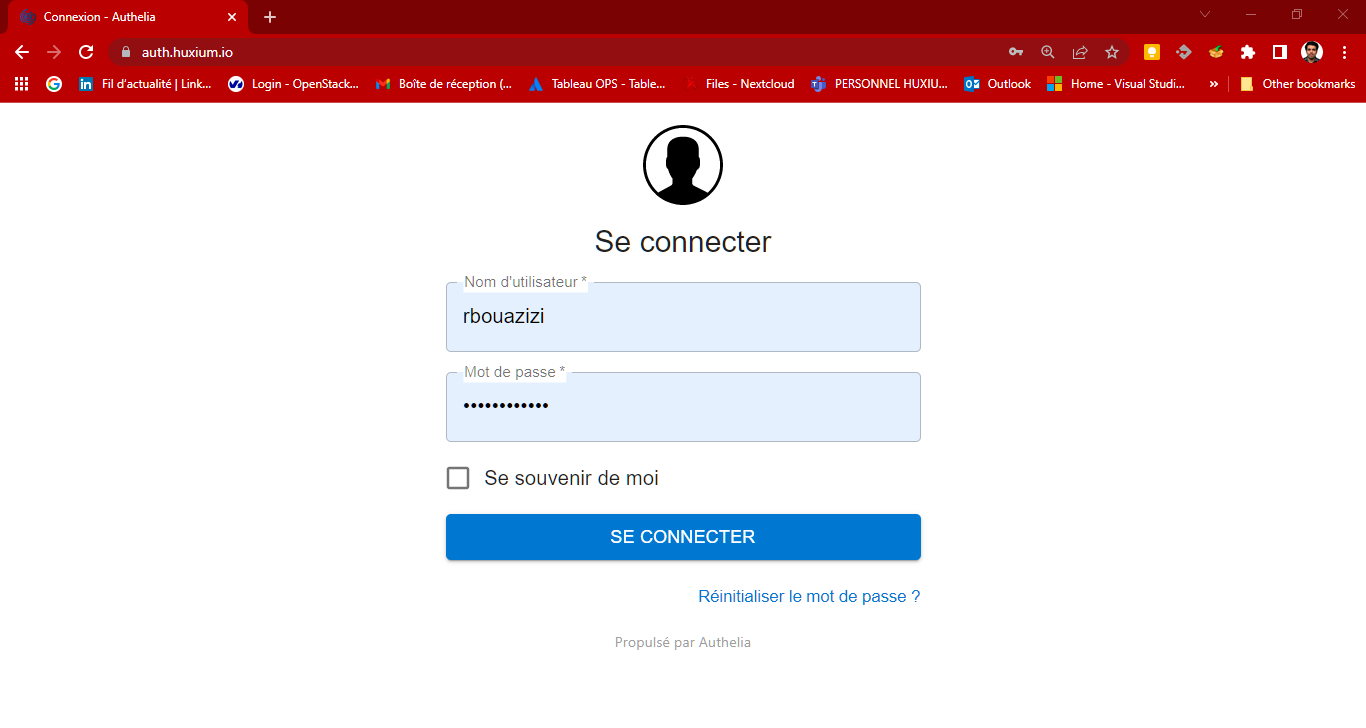
\includegraphics[width=1.0\textwidth,angle=00]{assets/f55.png}
\caption{Authentication portal}
\label{fig:f55}
\end{figure}

\subsubsubsection{How it works }

The architecture works as follows: 
\begin{itemize}[label={--}]
\item The user sends a request to access a protected resource. 
\item  Traefik receives the request and forwards it to Authelia. 
\item  Authelia authenticates the user against the OpenLDAP server and checks the user's group membership to determine whether access is authorized. 
\item  If the user is authenticated and authorized, Authelia sets up a session for the user and sends a token to Traefik. 
\item  Traefik receives the token and sets it as a cookie in the user's browser for subsequent requests. 
\item  For subsequent requests, Traefik checks the cookie for a valid token and forwards the request to the backend service if the token is valid. Otherwise, the user is redirected to the authentication page.  
\end{itemize}